\makeheading{
回顾塑造了2019年的科学事件\\[-0.3em]The science news events that shaped 2019
}
\begin{multicols}{3}
\section*{遥望太空 Staring into space}

今年,神秘的黑洞首次现真容。4月,事件视界望远镜(\textit{Event Horizon Telescope}, EHT)公布了有史以来首张直接拍摄到的黑洞及其事件视界的照片,这或是今年最令人难忘的照片。为捕捉这张照片,世界各地的天文学家构建了一个口径相当于地球直径的望远镜阵列,从各地同时观测。

This year, astronomers \textit{glimpsed(瞥见)} the blackness of a black hole for the first time ever. In April, the international Event Horizon Telescope collaboration unveiled perhaps the most memorable picture of 2019: the first direct image of a black hole and its event horizon. To produce it, researchers coaxed a network of radio telescopes to take \textit{simultaneous(同时的)} readings from around Earth.

\begin{figure}[H]
    \centering
    \includegraphics[width=\linewidth]{IMG/202001/eso1907a.jpg}
    \caption{\textit{黑洞及其事件视界}}
    \label{fig:my_label}
\end{figure}


2019年也是阿波罗登月50周年,各国航天局将月球探索提上了议事日程。1月,中国的“嫦娥四号”探测器成为首个在月球背面安全着陆的航天器,“嫦娥四号”的月球车“玉兔二号”在冯·卡门撞击坑继续进行执行探测任务。

In a year that marked the 50th anniversary of the Apollo Moon landings, lunar exploration was high on the \textit{agendas(日程)} of space agencies. In January, China's Chang'e-4 probe became the first spacecraft to land safely on the lunar far side. Its rover, Yutu-2, continues to roll across the dusty soils of Von Kármán crater. 

\begin{figure}[H]
    \centering
    \includegraphics[height=0.3\linewidth]{IMG/202001/6782939.jpg}\hfill\includegraphics[height=0.3\linewidth]{IMG/202001/6782940.jpg}
    \caption{\textit{嫦娥四号与玉兔二号}}
    \label{fig:my_label}
\end{figure}

正在进行的火星任务返回了一系列结果。美国宇航局(NASA)的“洞察号”探测器探测到了人类历史上的首次“火星震”,该探测器配备了由法国制造的地震仪。6月,大约600公里之外的NASA“好奇号”探测器探测到火星大气中的甲烷气体浓度创下历史新高,目前科学家对此无法做出解释,更奇怪的是这般高浓度的甲烷气体几天后消失了。2月,NASA宣告“机遇号”火星探测器正式退役。


Ongoing Mars missions returned a host of results. The French-built \textit{seismometer(地震仪)} on NASA's InSight lander detected the first-ever ‘marsquakes’. Roughly 600 km away, NASA's Curiosity rover \textit{sniffed(嗅)} record-high levels of \textit{methane gas(甲烷)} in the Martian atmosphere in June — a mystery that scientists have yet to explain, especially because the methane \textit{vanished(消失)} in days. In February, NASA officially bid farewell to its most stalwart Mars rover, Opportunity.


让我们把目光望向太阳系的更远端。2月,日本的“隼鸟2号”探测器在从小行星“龙宫”表面进行了样本采集。7月,它向龙宫发射弹丸撞击其表面,并着陆采集经撞击后露出的一些物质,并将于明年将样本送回地球。


In the farther reaches of the Solar System, Japan's Hayabusa 2 probe collected a sample from the surface of the asteroid Ryugu in February. Then, in July, it dropped a small \textit{pellet(弹丸)} onto the asteroid and \textit{blasted(撞击)} its surface, before descending to gather some of the freshly exposed material, and will return its samples to Earth next year. 

今年还有一位闯入太阳系的星际来客。12月上旬,星际彗星2I/Borisov掠过太阳,这是继2017年神秘的星际访客奥陌陌(\textit{`Oumuamua'})之后,已知的第二颗从另一星系造访太阳系的天体。

This year even brought a visitor from beyond the Solar System. The interstellar Comet 2I/Borisov \textit{whizzed(略过)} past the Sun earlier this month. It is only the second object known to have visited our Solar System from another one, following 2017's `Oumuamua'.

\section*{量子奇迹 Quantum wonders}

经过漫长的等待,物理学家终于在量子计算领域迎来了新的里程碑。谷歌的一个团队使用量子计算机进行了一项特殊的计算。而这项计算对甚至对最先进的超级计算机而言,几乎都是不可能的。这项计算本身是用于检查量子随机数发生器的输出,虽然其实际用途有限,但这一壮举是量子计算机向未来应用迈出的一步,其实际用途覆盖了从设计新材料到破译密码的各种领域。

Physicists reached a long-awaited milestone in \textit{quantum(量子)} computing. In October, a team at Google used a quantum computer to perform a calculation that would be practically impossible for a classical machine, even a \textit{state-of-the-art(最先进的)} supercomputer. The calculation itself — checking the outputs from a quantum random-number generator — is of limited practical use, but the \textit{feat(成就)} is a step towards future applications of quantum computers, which range from designing new materials to codebreaking.

\begin{figure}[H]
    \centering
    \includegraphics[width=\linewidth]{IMG/202001/1024.jpg}
    \caption{\kaishu 谷歌的Sycamore量子处理器}
    \label{fig:my_label}
\end{figure}

今年早些时候,化学家利用原子力显微镜操纵单个分子,制造出人类历史上首个环状纯碳分子,分子尺度晶体管由此进入了大众视野。

Earlier in the year, molecular-scale \textit{transistors(晶体管)} came into view when chemists made the first-ever ring-shaped molecule of pure carbon by using an atomic-force microscope to manipulate individual molecules.


\section*{突破生物边界\\Pushing biological boundaries}

这是在实验室中检验生物学和伦理界限的一年。美国科研人员在猪的头部被砍下4小时后,通过泵入一种富含营养和氧气的液体来模拟血液,使其大脑成功复苏。这一操作触发了糖的消耗和其它代谢功能,表明大脑仍然在运作。

It was a year of testing biological and \textit{ethical(伦理)} limits in the laboratory. US researchers \textit{revived(复苏)} the brains of pigs four hours after their heads had been severed, by pumping in a nutrient- and oxygen-rich liquid to \textit{mimic(模拟)} blood. The trick triggered sugar consumption and other metabolic functions, suggesting that the brains were still working. 


日本继续在诱导多能干细胞的临床应用中占据主导地位,诱导多能干细胞是指被重编程为胚胎样状态的成体细胞。9月,日本的一个研究小组利用这些干细胞,造出了可以移植到视力衰退女性体内的角膜细胞片。过去十年里,日本医生已经在使用诱导多能干细胞治疗帕金森氏病和另一种眼部疾病。今年,一个研究小组被批准使用干细胞治疗脊髓损伤。但是这些治疗方法是否有效仍是未知数。

Japan continued its \textit{dominance(主导地位)} in the clinical use of induced pluripotent stem cells — adult cells that are reprogrammed into an embryonic-like state. In September, a Japanese group used these stem cells to make sheets of corneal cells that could be \textit{transplanted(移植)} into a woman whose eyesight was failing. In the past decade, Japanese physicians have used iPS cells to treat Parkinson's disease and another eye condition, and this year a group was granted approval to use stem cells as a therapy for spinal-cord injury.





\section*{胚胎编辑 Embryo edits}

2019年伊始,中国科学家贺建奎宣布了世界上首对基因编辑婴儿的诞生。消息一出,全世界一片哗然,至今影响仍在。他通过CRISPR/Cas9系统对CCR5基因进行了修改,使这对双胞胎女婴对HIV病毒产生抵抗力。在这之前,国家卫健委的一项调查发现,贺建奎违反了禁止将基因编辑用于生殖目的的国家规定。3月,国家卫健委发布了进一步的法规草案,其中包括对违反人类基因编辑规定的个人进行严厉处罚。当月,世界卫生组织的一个咨询委员会呼吁建立一个全球人类基因编辑研究登记处,并反对临床上在人体内应用可遗传的基因编辑。

As 2019 began, the world was still reeling from the announcement that Chinese scientist He Jiankui had produced the world's first gene-edited babies. He used the CRISPR–Cas9 system to alter the gene CCR5, in an attempt to give twin girls \textit{resistance(抵抗力)} to HIV. Chinese health-ministry found that he had violated national regulations forbidding the use of gene editing for reproductive purposes. In March, the health ministry issued further draft regulations that included severe penalties for those who break rules regarding gene editing in humans. That month, an advisory committee to the World Health Organization called for the creation of a global registry of human gene-editing studies, and opposed the clinical use of heritable gene editing in humans.

10月,博德研究所的化学生物学家David Liu领导的一个团队,公布了一种叫做先导编辑的方法。早期结果表明,这种替代工具可能比标准的CRISPR-Cas9编辑更精确,这可能会减少对人类使用基因编辑安全性的一些担忧。

In October, a team led by chemical biologist David Liu of the Broad Institute in Massachusetts, unveiled a method called \textit{prime(首先的)} editing. Early results suggest that this \textit{alternative(替代的)} tool could be more precise and accurate than standard CRISPR–Cas9 editing, which might \textit{ease(减轻)} some of the concerns about the safety of using gene editing in humans.\ \EOA
\end{multicols}
\ADyixuehui
\newpage
\makeheading{春节期间人口大量流动下的新冠肺炎疫情防控\\[-0.5em]{\LARGE COVID-19 control in China during mass population movements at New Year} }
\centerline{Simiao Chen, Juntao Yang, Weizhong Yang, Chen Wang, Till B\"anighausen\\
摘编自《柳叶刀》\textit{The Lancet} }
\begin{multicols}{3}

当前,新型冠状病毒肺炎 (COVID-19)疫情仍在中国持续扩 散蔓延疫情发展初期正值春节大量众 集中在春节期间返乡,形成全国大 规模的人口流动春运一般持续 40 天,在此期间全国客运量约达 30 亿 人次湖北省会武汉是此次疫情的重 灾区,500 多万人在 1 月 23 日封 城前就已离城,其中约三分之一流入 了外省减少这些人群的社会接触至 关重要,因为无症状或轻微症状的 COVID-19 患者仍具有传染性。 

The outbreak of novel coro- navirus disease 2019 (COVID-19) continues to spread rapidly in China. The Chinese New Year holiday \textit{coincided(同时发生)} with the emergence of COVID-19, during which a massive human \textit{migra- tion(迁徙) }takes place as individuals travel back to their hometowns. People in China are estimated to make close to 3 billion trips over the 40-day travel period, or Chunyun, of the Lunar New Year holiday. About 5 million people left Wuhan,3 the epi- centre of the COVID-19 \textit{epidemic(传染病)} before the start of the travel ban on Jan 23. About a third of those individuals travelled to lo- cations outside of Hubei province. Limiting the social contacts of these individuals was \textit{crucial(重要的)} for COVID-19 control, because patients with no or\textit{ mild(轻微的)}symptoms can spread the virus. 

\qiangdiao{中国政府在春节假期期间实施了一系列增加社会距离(social distancing)的措施,以减少人群间接触次数、增加人群间距离,这使得春节假期对于阻遏疫情蔓延可能起到一定作用。}

Government policies enacted during the Chinese Lunar New Year holiday are likely to have helped reduce the spread of the virus by decreasing contact and increasing physical distance between those who have COVID-19 and those who do not. 

这些举措包括鼓励居家休养,减少群众聚集性活动,取消或推迟大型公共活动,学校停课,部分政府机构停工,工厂停业;停运省际客运,仅保留部分城市公共交通系统。

As part of these social distancing policies, the Chinese Government encouraged people to stay at home; discouraged mass \textit{gatherings(聚集)}; cancelled or \textit{postponed(推迟)}large public events; and closed schools, universities, government offices,and factories.

得益于这一系列政策措施和健康宣传教育,广大人民群众普遍有了自我防护意识,尽量不出门、不集会、不聚餐,减少了人际接触,如必须出门亦会采取戴口罩等防护措施。

As a result of these policies and education campaigns, Chinese citizens started to take measures to protect themselves against COVID-19, such as staying at home, limiting social contacts, and wearing protective masks when they needed to move in public.

\qiangdiao{历史上抗击其它疫情的经验表明,增加社会距离措施能够有效遏制``人传人''的扩散,降低疫情发病率和死亡率。}虽然单个增加社会距离措施可以产生一定效果,但更常见的做法是将其与强制隔离等方式相结合,多措并举以增强防控效果。

Social distancing has been effective in past disease epidemics,\textit{ curbing (控制)}human-to-human transmission and reducing \textit{morbidity (发病率)}and \textit{mortality.(死亡率)}A single social distancing policy can cut epidemic spread, but usually multiple such policies---including more restrictive measures such as isolation and quarantine---are implemented in combination to boost effectiveness. 

政府和专家学者担心的是,1月31日春节假期结束后,全国范围内大规模的返工潮所带来的人群流动,极有可能会进一步加剧疫情蔓延。此外,春节后人员返程时间距离假期刚过一周,短于COVID-19最长潜伏期14日。在春节假期结束后,武汉封城前出城的500万人口中,有相当一部分可能还处于潜伏期内,而潜在感染者在春节假期结束后的大规模流动,必将对遏制疫情造成一定的困难。

During the current outbreak of COVID-19, government officials and researchers were concerned that the mass movement of people at the end of the Lunar New Year holiday on Jan 31, 2020, would\textit{ exacerbate(加剧) }the spread of COVID-19 across China. Moreover, individuals typically return from their Lunar New Year holiday after only 1 week, which is shorter than the longest suspected \textit{incubation period(潜伏期) }of the disease.~Many of the 5 million people who left Wuhan before the travel ban was put into place could still have been \textit{latently(潜在的) }infected when their holiday ended. This situation, together with the resumed travel activities, would make it difficult to contain the outbreak.

基于以上考虑,\qiangdiao{政府延长了春节假期},以使假期时长超过最长14日的潜伏期;同时将确诊病人在医院进行隔离。在感染人数最多的武汉,轻症确诊患者被隔离在由大型建筑(如体育馆或会议展览中心)迅速转型而来的大规模临时医疗场所,即``方舱医院''。

Facing these concerns, the Chinese Government extended the Lunar New Year holiday, so that the duration of the holiday would be \textit{sufficiently (足够)}long to fully cover the suspected incubation period of COVID-19.In addition, people \textit{diagnosed with(确诊)}COVID-19 were isolated in hospitals. In Wuhan, where the largest number of infected people live, those with mild and \textit{asymptomatic(轻症) }infection were also quarantined in so-called shelter or ``Fang Cang'' hospitals, which are public spaces such as stadiums and conference centres that have been repurposed for medical care. 

此外,政府充分发挥社区动员能力,追踪密切接触者,做到对患者的尽早发现与收治;通过社交媒体进行科普,鼓励公众勤洗手、勤消毒、出门戴口罩。通过实施这些政策,许多由湖北省前往其它省份的无症状感染者在出现症状前已处于隔离状态,出现症状后即接受治疗。对有湖北省旅行经历的人群进行居家隔离,可能是遏制病毒蔓延的最有效举措。

Finally, the Chinese Government encouraged and supported\textit{ grassroots(社区的) }activities for routine screening, contact tracing, and early detection and medical care of COVID-19 patients, and it promoted hand washing, surface disinfection, and the use of masks through social media. As a result of these measures, many people with asymptomatic infection from Hubei province who had travelled to other provinces remained in their homes until they developed symptoms, at which point they received treatment. It is this home-based quarantine of people who had been to the epicentre of the epidemic that is likely to have been especially helpful in curbing the spread of the virus to the wider community.

延长春节假期的举措可得到一些经验启示。\qiangdiao{首先,其他面临COVID-19潜在传播的国家,或是在未来应对其他突发传染病疫情时,可考虑将``控疫假期''或``控疫停工停学期''作为增加社会距离、降低疾病传染率的首选措施。}例如,在一段时间内关闭非生活必需的工作场所和公共设施。

There are several lessons that can be drawn from China's \textit{extension(延长) }of the Lunar New Year holiday. First, countries facing potential spread of COVID-19, or a similar outbreak in the future, should consider outbreak- control ``holidays'' or closure periods---ie, periods of recommended or \textit{mandatory(必要的) }closure of non-essential workplaces and public institutions---as a first-line social distancing measure to slow the rate of transmission. 

\qiangdiao{其次,``控疫假期''时长的确定,应考虑到该新发传染病的流行特征,例如潜伏期和传播途径。第三,``控疫假期''的核心是在整个停工停学期,防止潜伏期无症状感染人群传播疾病。}因此,政府应充分利用``控疫假期''进行防控知识的宣传教育,严格执行社区排查等措施,及时追踪管理密切接触者,使各项举措的效果最大化。

Second, governments should \textit{tailor(量身定制)}the design of such outbreak-control closure periods to the specific epidemic characteristics of the novel disease, such as the incubation period and\textit{ transmission routes(传染途径)}. Third, a central goal of an outbreak-control closure period is to prevent people with asymptomatic infections from spreading the disease. As such, governments should use the closure period for information and\textit{ education campaigns(公众宣传教育)}, community screening, active contact tracing, and\textit{ isolation(隔离) }and quarantine to maximize impact.

\qiangdiao{研究表明,增加社会距离与其它干预措施的结合使用能更为有效地降低疾病传染率,这为疫情防控多措并举提供了理论支持。}

Such a combination\textit{ approach(措施) }is also supported by studies of responses to previous outbreaks, which showed that reductions in the cumulative attack rate were more \textit{pronounced(显著的) }when social distancing policies were \textit{combined (结合)}with other epidemic control measures to block transmission. 

\qiangdiao{中国在抗击疫情的过程中,将``控疫假期''与其它措施结合使用,对遏制疫情蔓延起到了一定的作用,}这从湖北以外的省份每天新增确诊病例已连续下降两周多可见一斑。\qiangdiao{随着人们逐渐返工,政府应继续执行部分政策来确保持续防控此次新型冠状病毒肺炎疫情。}

As for COVID-19 in China, this combination of an outbreak-control closure period for social distancing and a range of accompanying epidemic control measures seems to have prevented new infections, especially in provinces other than Hubei, where new infections have been declining for more than 2 weeks. As travel and work slowly resume in China, the country should consider at least \textit{partial(部分) }continuation of these policies to ensure that the COVID-19 outbreak is\textit{ sustainably(持续) }controlled.\ \EOA

\mbox{}\hfill\textit{(全文有删改)}
\end{multicols}
\newpage
\makeheading{新药怎样从实验室走向市场}
\begin{multicols}{3}
\greyboxNID{\kaishu
\qiangdiao{导读}· 2月15日,在国务院联防联控机制新闻发布会上,科技部生物中心主任张新民表示,目前已遴选出5000个可能有效的药物作为候选药物,在普通冠状病毒感染的细胞水平上进行初筛,之后选定100个左右药物在体外开展活性实验。在这一基础上,科研攻关组聚焦少数几种药物开展临床试验,目前部分药物已显示出比较好的临床疗效。 

  新型冠状病毒肺炎疫情牵动着每个中华儿女的心。有同学不免发出这样的疑问:针对这次新型冠状病毒的特效药怎样研发?}

大家都希望能尽快研制出有效的药物来对付这“不速之客”。但是,我们必须要认识到,药物的研发、生产、应用有基本的规律和时间要求。
                                             
 


以传统的小分子化学药物为例,新药研发从无到有,要历经药物发现、临床前研究和临床试验“三部曲”,最后才能进入市场用于治疗疾病。细说起来可谓步步荆棘,成功者凤毛麟角。



\section*{第一步\quad 发现候选新药}

候选药物的发现首先需要选择和确定药物的作用\qiangdiao{靶标}。靶标是一种与某种疾病发生发展密切相关的生物分子,如蛋白和核酸等,对这种生物分子进行干预,能够治愈或缓解与其相关的疾病。

对于这次的新型冠状病毒而言,准确的药物作用靶标在哪里?

\begin{figure}[H]
    \centering
    \includegraphics[width=\linewidth]{IMG/202001/ncovmpro.jpg}
    \caption{\kaishu 2019新冠病毒的Mpro晶体结构}
    \label{fig:my_label}
\end{figure}

由蒋华良院士和饶子和院士领衔的应急攻关团队快速表达了新型冠状病毒水解酶(Mpro)并获得了它的高分辨率晶体结构,从而在此基础上进行药物的筛选。李华教授、陈丽霞教授等组成联合攻关小组,发现了冠状病毒nsp3编码的木瓜样蛋白酶(\textit{papain-like protease},PLP)在病毒基因组复制及逃避宿主抗病毒天然免疫中发挥重要作用,是药物开发的良好靶点。更多科学家目前正在寻找更多可能抑制新型冠状病毒的药物靶点,为抗新型冠状病毒肺炎药物的研发提供更多指导信息。

\qiangdiao{药物作用的靶标确定之后,药物化学家们需要根据靶标的空间结构,设计或者合成有作用的先导化合物。}这些化合物可以是全新结构的化合物,也可以来自天然产物(\textit{动物、植物、海洋生物}),甚至还可以是一些已经上市的药物。

经活性筛选得到先导化合物后,还需要以先导化合物为模板合成大量的新化合物,进一步筛选优化得到活性更好的化合物;同时,仍需系统地研究化合物的理化性质,代谢性质以及毒理早期数据,才能筛选出来满足成药性的最优化合物,这时候可以作为候选药物,进入临床前开发。

\section*{第二步\quad 候选新药临床前研究}

接下来新药就从研究进入了开发阶段,也就是系统的临床前和临床研究工作,这时候需要大量的资金投入。

临床前研究需要进行包括\qiangdiao{原料药的药学研究,动物体内的药理药效,药代动力学,以及安全性评价在内的系统研究工作,而这部分研究需要在动物身上进行。}

\noindent\qiangdiao{药学研究}\quad 早期合成的原料药主要用于药效、药代、早期毒理等的研究,从而充分地评价药物及其相关杂质的安全性。

随着新药研发进入后面的临床阶段,药物化学家们还得不断放大合成规模,优化生产工艺,逐步满足商业化生产的需求。


\noindent\qiangdiao{药效学研究\quad}这阶段主要是为了解答药物作用的机制,包括了解药物多大剂量起效,以及在什么时候有效,对什么人群有效等相关科学问题,从而确定药物的给药剂量和频率等关键信息。

而解决这些问题的前提,是要找到是找到合适的分子、细胞进行体外药效评价,并构建对症的动物模型进行体内药效评价。而对症的动物模型往往容易成为新药研发的瓶颈。对于新型冠状病毒肺炎,加快新药研发的步伐离不开对症动物模型的尽早建立。

\noindent\qiangdiao{药代动力学研究\quad}研究药物在动物体内的吸收、分布、代谢、排泄的性质(ADME),从而指导临床研究以何种形式给药(\textit{口服 注射 吸入等})。另一方面,药代动力学也有助于确定新药的给药频率和剂量。

\noindent\qiangdiao{安全性评价\quad}一般需要在至少两种动物种属(\textit{例如大鼠和犬})中进行评价,包括急毒,长期毒性,安全药理,遗传毒性,致癌性,致敏性,依赖性等,从而获得毒性靶器官,最大耐受剂量,等关键结果。这些毒性评价的结果可为确定新药的首次人体试验的起始剂量提供依据,并为制定人体临床试验的风险防控措施提供依据。

\section*{第三步\quad 临床研究}

\qiangdiao{临床阶段需要在人体上进行试验,因此药物进入临床研究前必须得到国家药品监督管理部门的审批。}在中国,新药的研发机构需要向国家药品监督管理局(\textit{National Medical Products Administration}, NMPA)提交新药临床申请(\textit{Investigational New Drug}, IND),获得许可后才能进行人体临床试验。

临床研究还需要分为四个阶段:

\noindent\qiangdiao{\uppercase\expandafter{\romannumeral1} 期临床试验}\quad 在健康志愿者身上研究新药在人体内的安全耐受性和药物代谢性质的试验,为制定给药方案和推荐安全剂量提供依据。

\noindent\qiangdiao{\uppercase\expandafter{\romannumeral2} 期临床试验}\quad 在真正的患者身上进行临床试验,主要目的是获得药物治疗的有效性数据,以及进一步的安全性数据,一般这个时候可以明确具体的适应症。

\noindent\qiangdiao{\uppercase\expandafter{\romannumeral3} 期临床试验}\quad 在更大范围的病人志愿者身上进行扩大的多中心临床试验,是治疗作用的确证阶段,也是决定药物研发是否能够成功的关键阶段。

\noindent\qiangdiao{新药上市申请}\quad 在完成了上面三个阶段的临床试验后,对临床数据进行统计学分析,证明药物安全有效的同时,确保新药安全,有效,可控这三点都符合要求后,药企或研发机构向药监部门提交新药上市申请(\textit{New drug application}, NDA)。获得药监部门批准后,新药才可上市销售,供医生和病人选择。

\noindent\qiangdiao{\uppercase\expandafter{\romannumeral4} 期临床试验}\quad 药物上市后,监测药物的长期副作用等情况。如果新药上市后发现了新的严重不良反应,该药有可能会被药监部门撤市。




难道在新冠肺炎疫情的紧急关头,我们不能缩短药物研发的时间和标准吗?

答案是:\qiangdiao{我们可以加快研发速度,但仍要遵循新药研发规律。}药物的研发是一项周期长,投资高,风险大的系统工程,每一个环节都来不得半点错误,否则人命关天。

\noindent\qiangdiao{周期长\quad}一个创新药物从实验室研究到最终上市可能需要10年;

\noindent\qiangdiao{投资高\quad}据不完全统计,全球的各大制药公司对于一个创新药物的资金投入,从最初到研发上市花费金额平均高达20多亿美元;

\noindent\qiangdiao{风险大\quad}导致药物研发失败的原因有很多,如在人体内的有效性不够、人体无法耐受或有严重毒副作用等。从实验室研发出潜在有效的化合物只有约万分之一能够最终有效投入市场。

对于已经上市或者国内外正处于临床试验阶段的药物,如若增加新的适应症,如把抗埃博拉病毒的药物用于治疗新冠肺炎,也需要经过系统的临床试验研究才能确定能否用于该新适应症。此外,还需与药监局进行沟通,并须得到药监局的许可才能进行相关的临床试验。

由于新型冠状病毒和同为冠状病毒的SARS、MERS有类似之处,相比17年前的SARS,科学家们对新型冠状病毒肺炎的研究和理解要深入得多,某些程度上可能会缩减药物研发的时间。但是,\qiangdiao{新药开发的规律无法被逾越。药物研发这事,急不得。}\EOA

\end{multicols}
\ADxinhangdao\vskip-5em
\makeheading{新冠肺炎与美国流感的区别与共性}

\begin{multicols}{3}
\greyboxNID{\kaishu
\qiangdiao{导读}·新型冠状病毒(2019-nCoV)感染引发的肺炎疫情(COVID-19)牵动着中国人民的心,而与此同时,在大洋彼岸,另一起疫情也引起了人们的关注。美国的流感季如期而至。根据美国疾病控制与预防中心(CDC)发布的数据,此次流感季中预计有2200万$\sim$\ 3100万人受感染,因流感死亡的患者人数在1.2万$\sim$\ 3万人之间。看到这样的数字,同学们可能会想,难道美国的流感疫情更严重?事实果真如此吗?COVID-19与流感疫情相比,又有哪些差异?}

\section*{未知的风险}
流感病毒(\textit{包括甲型和乙型流感病毒})和2019-nCoV都属于可引起呼吸道疾病的病毒。需要提醒的是,\qiangdiao{流感虽然被称为流行性感冒,但却与普通感冒关系甚远。}流感是由一类特殊的流感病毒引起的,相比普通感冒,它的致病源不同,因此也就具有更强的传染性和更高的致死率。

在公共卫生领域,两者最大的差异就是\qiangdiao{人类的认知程度}\qiangdiao{。}对于流感病毒,科学家已经研究了数十年,因此流感虽然危险,但我们对流感的治疗手段、发病症状以及可能的流感暴发季节都有着充足的了解。相比之下,我们对这种全新的新型冠状病毒(2019-nCoV)的了解却很少。对于其将来的传播范围、造成的死亡人数、疫情最终的结果,人们很难预知。这种未知,也是我们恐惧的源头之一。

美国过敏和传染病研究所(NIAID)所长安东尼$\cdot $福奇(Anthony 
Fauci)在白宫的新闻发布会上表示:``尽管流感的发病率和死亡人数也很高,但我们已经摸清楚了流感的暴发规律。我可以向你们保证,到了3、4月,流感患者数量就会减少。事实上,我们能够非常准确地预测出季节性流感死亡率和住院人数的大致范围。但现在的问题在于,2019-nCoV仍有很多的未知数。''

除此之外,两种病毒在病毒传播、临床症状与治疗等方面也存在诸多差异。对于2019-nCoV,科学家正竞相发掘更多信息。

\section*{传染能力}
此次疫情蔓延迅速的一项重要原因,就是2019-nCoV强大的传染能力。科学家常常用\qiangdiao{``基本传染数''($\mathbf{{ R_0}}$)}来评估病毒传播的难易程度。通俗地说,就是评估一名感染了某种传染病的患者,平均能够传染给多少人。$R_0$值越高,这种传染病的传染能力越强。

而对于2019-nCoV的$R_0$,研究人员仍在努力确定。1月29日发表于《新英格兰医学杂志》上的一项研究估计,新型冠状病毒的$R_0$值约为2.2。但也有研究指出,\qiangdiao{2019-nCoV的$\mathbf{{ R_0}}$达到3.77}。也就是说,平均每个受感染的人能将这种病毒传染给3.77个人。\qiangdiao{如果这一结论得到确认,这意味着2019-nCoV的传染能力远超此前的预期。}

需要注意的是,每种疾病的$R_0$并不是一个固定的常数。$R_0$因地区而异,具体取决于人们相互接触的频率,以及防疫措施的强度。

病毒潜伏期的长短,也是影响疾病传染能力的重要因素。流感病毒的潜伏期多在1$\sim 
$4天,而2019-nCoV则更加复杂。根据钟南山院士领衔发表在预印本网站的一项回顾性研究,2019-nCoV潜伏期的中位数为3天,但不同患者间存在显著差异:患者最快在当天发病,而一名患者自称经过24天的潜伏期才显现出症状。潜伏期较长的患者,对早期的诊断与隔离提出了挑战。

\section*{传染方式}
流感病毒的人与人传染主要通过三种方式实现:

\noindent\qiangdiao{直接传播}\quad 也称飞沫传播,指患者打喷嚏、咳嗽或说话时产生的飞沫,被周围的人吸入体内导致的感染。

\noindent\qiangdiao{气溶胶传播}\quad 飞沫混合在空气中,形成气溶胶,吸入后导致感染。

\noindent\qiangdiao{接触传播}\quad 飞沫沉降在物品表面,手部接触污染源后,再用手接触口腔、鼻腔、眼睛等部位的粘膜,导致感染。

流感病毒附着在呼吸道内细胞上,然后,流感病毒的血凝素表面蛋白与人呼吸道细胞表面的唾液酸受体结合,从而打开人类细胞的``锁'',进入并感染细胞。

\section*{症状和严重程度}
根据美国疾病控制与预防中心(CDC)的报告,流感的典型症状包括发烧、咳嗽、咽喉痛、肌肉酸痛、头痛、流涕或鼻塞、浑身乏力以及偶发的呕吐或腹泻。流感的症状通常是突然发作的,大多数流感病毒的感染者会在两个星期内康复。但对一小部分人来说,流感病毒还会引发其他并发症,比如肺炎。

在美国,2019-2020年的流感季已经造成了\qiangdiao{2200万$\sim 
$3100万人感染,1.2万$\sim 
$3万人死亡,}但\qiangdiao{致死率不到0.1{\%}}。此外,到目前为止,这个流感季中大约1{\%}感染者的症状程度需要住院,这一比例与上一个流感季相近。

\begin{figure}[H]
\centerline{\includegraphics[width=\linewidth]{IMG/202001/新型冠状病毒肺炎VS美国流感11.png}}
\label{fig1}
\end{figure}

需要指出的是,美国流感感染者、死亡人数等数据不是通过直接统计得出,而是\qiangdiao{基于美国CDC建立的动态模型的评估结果。}这个模型通过全美13个流感监测点,覆盖的9{\%}的人口中的感染数、住院数、疫苗接种率、高危病例数以及死亡数等信息进行推演。这样做的原因是,一方面,大量流感患者可能不会前往医院,或是没有进行流感病毒检测;另一方面,一些人可能因流感导致的并发症(\textit{如肺炎、心血管疾病等}\textit{如肺炎、心血管疾病等})死亡,对于这些人,医院统计的直接死因并非流感,但流感却是其去世的诱因。从中可以看出,\qiangdiao{美国CDC对于流感死亡人数的统计范围也更加宽泛},这也部分解释了美国每年因流感死亡的人数都达到数万人。

对于2019-nCoV感染的症状和严重程度,人们正试图深入了解。钟南山院士团队在最新研究中分析指出,COVID-19最普遍的症状是发热和咳嗽,腹泻、呕吐等消化系统的症状极为罕见。此前发表于《柳叶刀》的一项研究也显示,只有约5{\%}的患者表现出了喉痛和流涕的症状。相比之下,COVID-19的严重程度远超流感。根据世界卫生组织(WHO)2月4日发布的数据,在中国报告的2万余例患者中,约有14{\%}为重症患者。

\qiangdiao{综合现有研究的判断,2019-nCoV感染的致死率约在1{\%}$\sim 
$3{\%}之间,远高于流感。}不过,随着疫情的进一步发展,这一数字还可能发生变化。美国卫生与公共服务部部长在1月28日的新闻发布会上表示,在疫情暴发初期,最初发现的病例可能存在``严重倾斜''。也就是说,最初确诊的病例可能大多是较为严重的患者,这可能会导致计算出的死亡率高于实际水平。随着更多轻症患者得到确诊,死亡率可能会下降。

\section*{预防与治疗}
我们可以通过注射疫苗来预防60{\%}的季节性流感。目前,针对COVID-19的疫苗研发工作正在进行中。一些国内外团队已经进入动物试验阶段,不过距离疫苗的最终问世,仍需较长的时间。(\textit{见本期“新药怎样从实验室走向市场”})

对于流感,人们已经找到了较为有效的抗病毒药物。对于本季的流感,美国CDC的推荐药物包括奥司他韦,扎那米韦和帕拉米韦等。而在COVID-19的临床治疗中,静脉注射抗生素、氧气治疗、奥司他韦与机械通气是目前使用较为频繁的几种疗法。此外,有较多的重症患者接受了全身性糖皮质类固醇治疗。针对COVID-19的特效药仍在寻找中。瑞德西韦的临床试验正在武汉的医院内进行中,此外阿比朵尔、达芦那韦等药物在体外细胞实验中也展现出潜力。但距离药物通过临床测试上市,同样需要一段时间。

无论是流感还是新冠肺炎,下面的建议是通用的:经常用清水和香皂洗手,洗手时间不短于20秒钟;不要用未洗的手触摸眼睛、鼻子和嘴巴等部位;避免与患者密切接触;不要到处走动或去人员密集的区域;以及注意清洁和消毒经常触摸的物体或表面。\EOA
\end{multicols}
\ADhairui
\newpage
\makeheading{生活中的科学·上期答案}

\begin{multicols}{2}
\noindent\qiangdiao{Q1为什么空杯子或者花瓶放到耳边会有声音?}

外部的白噪音在共振腔中集中放大了某些频率的声音,而空杯子和耳朵之间形成了共振腔。外部的噪音通过共振腔在空气作用下集中了某些频率的声音(\textit{频率和共振腔的几何外形相关}),相当于外部的噪音是这些声音的演奏者。因此,如果我们可以将外部白噪音和共振腔完全隔绝,阻止空气振动的传播,就听不到上述的声音了。

如果尝试站在嘈杂的大街和待在下雪天的家中,再将空杯子凑在耳朵边,你就会发现后者听到的声音明显变小了。

\noindent\qiangdiao{Q2为什么冷水冲不开咖啡?热水冲开之后不会沉淀?}

冲泡咖啡的过程是一个咖啡溶解于水的溶解过程。影响溶解的因素有很多,温度就是其中之一。一般来说,温度越高,溶解越快。这是因为温度越高,分子热运动加剧,咖啡分子移动到水分子之间的空隙中也越容易,宏观上的体现便是咖啡溶解。冷水创造出的低温环境会减缓这个过程,但并不是不能完成。热水冲开咖啡之后不会沉淀,便要涉及到溶解度的问题。溶解度是一定温度下每100g水中能溶解溶质(\textit{咖啡})的克数。要想溶解后出现沉淀,则需要达到饱和即最大溶解度之后再加入溶质(\textit{咖啡}),才能析出溶质(\textit{咖啡})。

\noindent\qiangdiao{Q3 为啥自行车车胎充气后骑着轻,没气时重?}

理想情况下,自行车在公路上行驶不需要外力驱动。实际情况下并不能满足理想条件。当自行车胎没气时,行驶过程中车胎一直处在被压扁-释放-压扁-释放的状态,这个过程造成大量的机械能转化成内能,能量利用率降低,所以骑起来会变重。

那为什么不直接去掉车胎呢?答案很简单,如果去掉车胎,轮毂和地面就形成刚性接触,受力非常不均匀,容易造成轮毂损伤,骑车者会觉得振动非常大,减弱骑行体验。轮胎还可以增加车轮和地面的摩擦力,减少打滑。

\noindent\qiangdiao{Q4 为什么会形成白色的浪花?}

我们都知道,水是无色透明的,而海洋是蓝色的。那么为什么海洋是蓝色的呢?因为海水发生瑞利散射的原因,大海在我们的眼里是蓝色的。

那为什么浪花是白色的呢?首先,浪花的组成成分不仅仅有水,还有气泡,这些气泡对浪花的颜色有着至关重要的影响。气泡的表面是膜状的,上面的小水珠就像一个个棱镜;当光线照在浪花上的时候,浪花表面会发生多次的反射以及折射,最终光线从不同方向反射出来。而由于各种颜色的光反射概率相等,导致最终变成了我们所熟悉的白色的浪花。\EOA
\end{multicols}
\vskip-3em
\makeheading{电脑里的A盘和B盘藏到哪里去了?}
\begin{multicols}{3}
当你无聊点开了桌面上的“此电脑”,你会看到C盘带着一众小弟躺在里面。大多数人不会考虑:为什么电脑的系统盘是C盘,不是A盘?要回答这个问题,我们就要回到过去,看看那些被历史淘汰的产品——软盘。

在系统默认的情况下,A盘指3.5英寸软盘,B盘则是5.25英寸软盘。最先进的3.5英寸软盘,容量只有1.44MB。就是这种现在连一首MP3都存不下的介质,装载着MS DOS系统打开了计算机的新世界。事实上,你仍然可以通过手动分配的方式让你的硬盘挂上“A:”、“B:”的盘符,但和真正的软盘相比,\qiangdiao{没内味}。

软盘早早退出了家用计算机的历史舞台,大概现在只有90后还见过它。据新华社报道,美军核弹部队截至2016年仍在使用最古老的8英寸软盘,美国国防部发言人瓦莱丽·亨德森介绍:“因为他们还没坏。”

1967年,IBM公司推出一款32英寸软盘,有一个公交车轮胎那么大。

\begin{figure}[H]
    \centering
    \includegraphics[width=\linewidth,clip=true,trim=0 140 0 0]{IMG/202001/floppy.jpg}
\end{figure}

1971年,Alan Shugart推出一种直径8英寸的表面涂有金属氧化物的塑料质磁盘,这就是我们常说的标准软盘的鼻祖,但它的容量只有81KB。

1976 年,Alan Shugart又推出了直径为 5.25 英寸的软盘,刚推出时储存容量也仅为 360 KB ,随着技术的成熟,最大容量可达 1.2 MB ,软盘也开始渐渐普及起来。

1980 年索尼推出了 3.5 英寸的软盘和软驱,尺寸变小,容量也变大为 1.44 MB ,不过 3.5 英寸软盘刚推出的时候,市面上的主流依然是 5.25 英寸软盘。

\begin{figure}[H]
    \centering
    \includegraphics[width=0.7\linewidth,clip=true,trim=0 0 10 0]{IMG/202001/0_1316582210EB43.jpg}
\end{figure}

软盘在使用之前必须要先格式化,完成这一过程后,磁盘被分成若干个磁道,每个磁道又分为若干个扇区,每个扇区存储512个字节。磁道是一组同心圆,一个磁道大约有零点几个毫米的宽度,数据就存储在这些磁道上。一个1.44MB的软盘,它有80个磁道,每个磁道有18个扇区,两面都可以存储数据。\EOA
\end{multicols}

\newpage
\makeheading{科技快讯}
\begin{multicols}{3}

\section*{长江白鲟宣告灭绝}

\noindent\includegraphics[width=\linewidth]{IMG/202001/cjbx.jpg}

长江白鲟(\textit{Psephurus gladius})是一种可以长到7米长的淡水鱼,已经被宣告灭绝。长江白鲟的吻形似一把长剑,里面满是电感应细胞,主要用来追踪猎物。1981年葛洲坝截流工程完工,白鲟与其长江上游唯一的产卵地被切断。据研究人员估计,1993年,长江白鲟就已经功能性灭绝,即其数量已经不够维持种群持续生存。“长江白鲟是第一个但不会是唯一一个灭绝的大型淡水鱼,其他很多鱼类都岌岌可危。”鱼类生物学家Zeb Hogan说。

\section*{人类平均体温正在下降}

\noindent\includegraphics[width=\linewidth]{IMG/202001/pjtw.jpg}
 
自1860年以来,人类的正常体温下降了约0.5°C。研究人员分析了1860年以来的数十万条体温测量结果,发现人类的平均体温每十年下降0.03°C。因为体温的测定方法本身存在许多未知的变量。事实上,可能并非所有人都相信这一令人难以置信的结果。但想想200年来人类生活的变化,体温的变化似乎也就变得不那么意外了。“回头看我们走过的19世纪,我敢肯定其中绝大多数人都存在慢性炎症性疾病。”传染病流行病学家Julie Parsonnet说。

\section*{太阳高清照片诞生}

\noindent\includegraphics[width=\linewidth]{IMG/202001/sun.png}

位于夏威夷顶的丹尼尔·K·伊努伊太阳望远镜(DKIST)是全球最大的太阳望远镜,直径4米,耗费3.44亿美元。经过7年的建设,DKIST在近期投入运行,并于1月28日发布了首张太阳近景照片,这也是太阳迄今最高分辨率的图像。图片中形似细胞的明亮结构代表从太阳内部喷射出的等离子体,而颜色较暗的是正在冷却、沉降的等离子体。DKIST将观测太阳磁场变化,帮助科学家理解太阳耀斑的形成机制,从而更好地预测太阳对地球的影响。\EOA
\end{multicols}\vskip-6em
\makeheading{课内知识拓展·定楼神器}
\begin{multicols}{3}
上学期我们学过了振动。用手指头我们也能想到,台风登陆的时候,空中的风速达到30-40 m/s。\qiangdiao{出现了!受迫振动!}要是和固有频率撞了,大楼不就开始共振么?虽说一般不会恰好与固有频率重合,大楼也具有钢筋不太可能会塌,但如果摇晃幅度太大,里面住的人也总感觉怪怪的......

1909年,弗拉姆提出了一种调谐质量阻尼器的概念。经过将近几十年的发展,它逐渐发展为我们现在在摩天大楼上普遍使用的调谐质量阻尼系统(TMD)。

\qiangdiao{在这里,我们把摩天大楼简化为竖直方向上受迫振动的弹簧振子模型。}大楼等效为$m_1$,在下面如果再用弹簧挂一个质量块$m_2$,我们就得到了一个调谐质量阻尼系统。我们发现,当系统整体的固有频率与驱动力频率相等时,$m_1$在外力作用下完全不振动,其能量完全转移给$m_2$。大部分情况,外力不会与之匹配,这时候将会形成一个双峰。原来只有一个频率振幅最大,你现在出现了两个,这不是我们想要的结果。

\noindent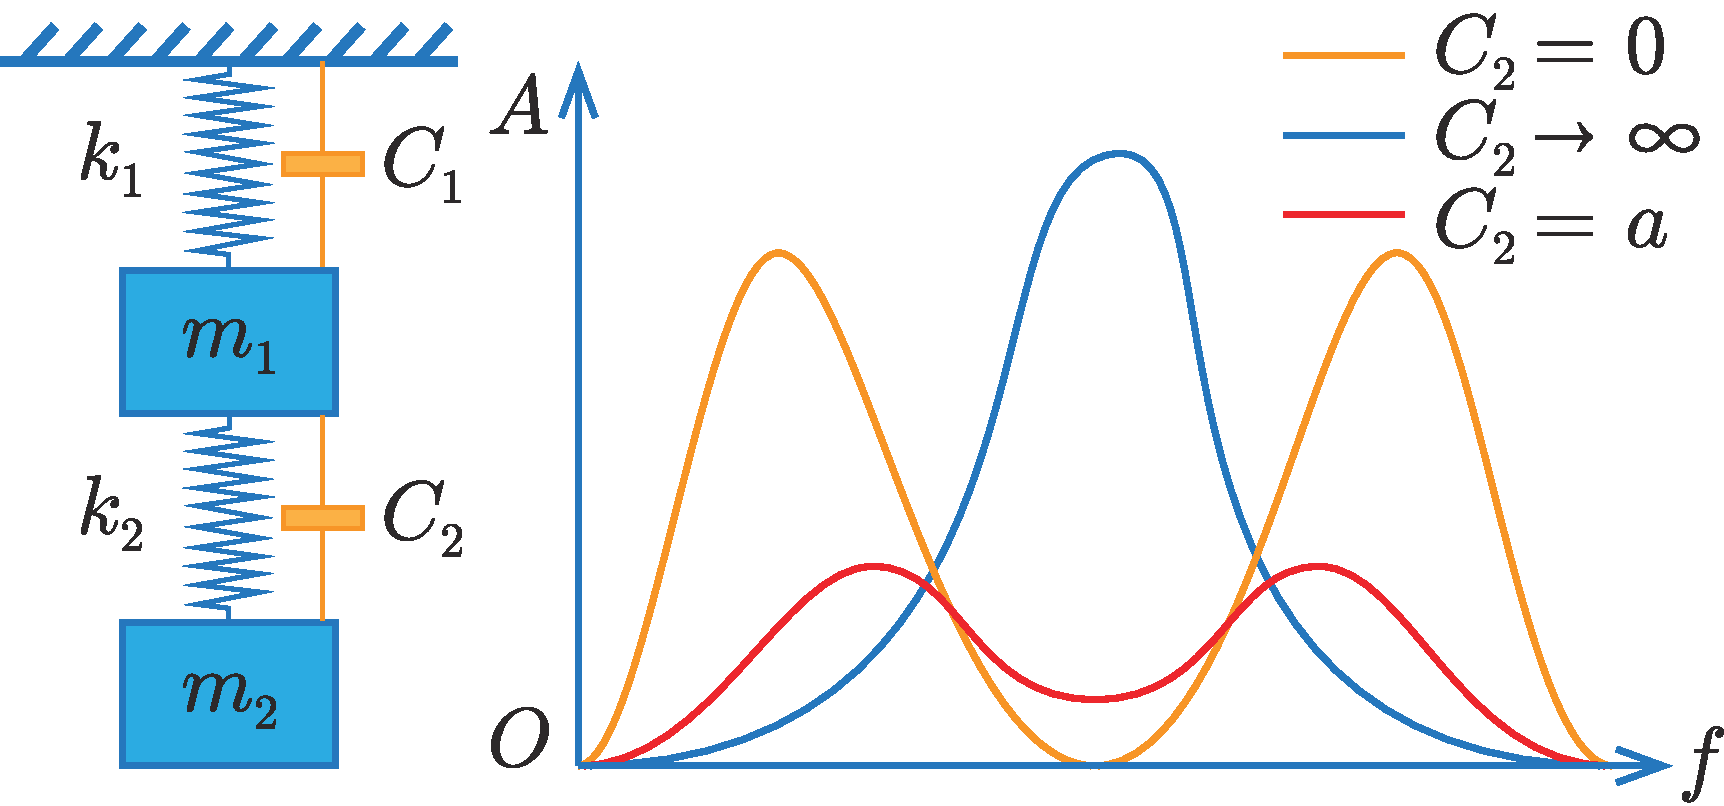
\includegraphics[width=\linewidth]{IMG/202001/DL.pdf}\vskip-0.5em

在不匹配的情况下,我们再考虑上大楼的阻尼$C_1$和质量块的阻尼$C_2$:在$C_1$一定时,我们调节$C_2$会发现:若质量块与大楼间没有阻尼,相当于上一段所述的情况,那就会出现明显的双峰现象;如果阻尼很大,直接刚性连接,相当于根本没有用弹簧加质量块,那么振动情况还是原来的单峰图象。\qiangdiao{$\mathbf{C_2}$在某个合适值$\mathbf{a}$下,系统整体振幅会在一定程度上减小。}这个数值可以根据公式计算得出,我们就不算了。由此,我们就可以领取我们自己的大楼了——

首先,我们调节$m_2$、$k_2$使质量块固有频率与大楼的固有频率相匹配,然后我们调节$C_2$到那个合适的数值,一套TMD系统就完成了。在这种情况下,$m_1$受迫的动能便会最大程度地转化为$m_2$的动能,在阻尼上被耗散掉了。

\noindent\includegraphics[width=\linewidth]{IMG/202001/tb101.jpg}

台北101大厦的风阻尼系统就是这样一套典型的TMD系统。在大楼的88-92层,四组钢索吊挂着一个直径5.5m,重约660t的质量块($m_2$)。质量块下方有一些油粘滞阻尼杆($C_2$),靠油的阻力耗散能量。其最大振幅可达1.5m。\EOA
\end{multicols}
\newpage
\makeheading{为什么神曲在我们脑中总是挥之不去?}

\begin{multicols}{3}

很多同学可能会有神曲“上头”的经历——即使没有在听歌,大脑里也会自动循环播放。这是为什么呢?难道我们大脑里装了一台立体环绕音响吗?


这种神曲在我们脑海里循环播放的现象有个好玩的名字,叫耳虫(\textit{Earworm}),由德文“Ohrwurm”借译过来。


\noindent\includegraphics[width=\linewidth]{IMG/202001/image001.jpg}
 

2007年,科学家们为“耳虫”现象下了一个新定义:不自主的音乐想象(\textit{involuntary musical imagery,简称}INMI),指某段音乐在脑中不断重复的现象。

这种情形无需刻意想象,便会在某一时刻突然出现在我们的脑海中,停留可长达数小时,甚至数日。尤其是当我们精神并未高度集中的情况下,如打扫卫生时,各种神曲就会突然弹出,然后我们就开始哼唱起脑子里的旋律。


这种现象极为常见。根据斯坦福大学的一项调查研究显示,在所有12000人的被调查者中,99\%的人都存在耳虫现象,而有90\%以上的人,每周至少会经历一次耳虫。

\section*{为什么这种现象会如此普遍?}

伦敦大学的音乐心理学家维奇•威廉姆森(Vicky Williamson)也表示自己就经常被耳虫现象困扰。她通过研究发现,耳虫现象可以用以下两个原因来解释。

首先,音乐可以用多种方式编排,不同乐器的混合会给我们多方面的感官刺激,最终使我们对这段音乐有了更加深刻的认识。此外,很多音乐都饱含了创作者的个性和情感,当我们感同身受时,会对这段音乐记忆尤深。

此外,人类的历史可追溯到几十万年前。在漫长的进化过程中,我们大部分时间都需要记住关乎生存的信息,如陷阱的位置,哪些食物能吃,哪些食物有毒等。相较于人类漫长的进化史,我们的书面文字却仅在5000年前产生。因此,我们的祖先可能通过歌曲的旋律来传递和记忆以上的生存信息,这也解释了我们会不由自主地记住一些音乐的原因。

耳虫现象虽然常见,但是每个人所受影响程度会有所不同,有的人很少出现,而有的人则深受影响。

\section*{什么样的人群更加容易出现耳虫现象?}

伦敦大学的神经学教授尼古拉斯• 法鲁吉亚(Nicolas Farrugia)及研究团队招募了44位经常出现耳虫现象的志愿者,并发放了问卷调查,内容包括耳虫现象出现的次数、频率,出现时的体验,以及是否会影响日常生活等;并收集了志愿者的脑部核磁数据,与其他正常数据进行对比分析。

分析显示,与耳虫出现频率低的人相比,这些经常出现耳虫的志愿者大脑皮层更厚,尤其是右侧哈氏回(\textit{Heschl's Gyrus}, HG)和右侧额下回(\textit{inferior frontal gyrus}, IFG),前者与听觉知觉和自主音乐想象密切相关,后者则参与了音调记忆的加工。

\noindent\includegraphics[width=\linewidth]{IMG/202001/image002.jpg}

此外,研究人员还发现,那些出现“耳虫”频率高的人,他们的右侧海马旁回皮层(\textit{parahippocampal cortex}, PHC)的灰质体积较大,而PHC的灰质体积增大有利于音乐相关的记忆和情绪的提取。


不过,研究人员表示,大脑的皮层厚度和灰质体积大小仅是个体间正常的生理结构差异,与大脑本身功能是否异常无关。此外,耳虫也不是病,对我们的健康也不会产生什么损害。但如果经常出现,会产生焦虑、失眠等后果。

\section*{当我们脑中经常出现神曲,挥之不去时该怎么应对?}

\qiangdiao{办法一,咀嚼口香糖. }此举可大大降低耳虫出现的概率。这是因为,咀嚼口香糖时,舌头与牙齿以及其他部位产生接合,这种开合运动降低了大脑对于音乐的记忆。



\qiangdiao{办法二,把神曲一次性听完. }根据研究显示,最容易导致耳虫现象的是20秒左右的音乐片段,这与当下短视频APP播放时长有异曲同工之妙。所以很多短视频网站的神曲就是利用这种片段侵袭了我们的大脑。\EOA
\end{multicols}
\noindent\parbox{0.655\linewidth}{
\greyboxNID{\vskip-5em
\makeheading{生活中的科学}
\vskip1em
 {Q1 }为什么用嘴吹气是凉的,用嘴哈气就是热的?

 {Q2 }用其它铅笔或中性笔涂机读答题卡可以被识别吗?

 {Q3 }顺风时,声音的传播速度会不会变快?

 {Q4 }为什么用钢笔在被水浸湿的纸上写字,写出的字会漾开?

 {Q5 }为什么空调要分制冷和制热呢?冬天开制冷25℃也会暖和吗?
\vskip1em
}}\hfill\parbox{0.305\linewidth}{\includegraphics[width=\linewidth,clip=true, trim=0 80 0 80]{IMG/202001/img-272cfeb00a40c9a09cc305f9fad5d934.jpg}\\\kaishu   吉林一号卫星在约600km高的轨道上拍摄到约420km轨道上的国际空间站\hfill\copyright 长光卫星}

\parbox{0.5\linewidth}{}